\documentclass[xcolor=svgnames]{beamer}
%\documentclass[xcolor=svgnames,handout]{beamer}
\usetheme{Boadilla}
\usecolortheme[named=ForestGreen]{structure}
\usepackage{graphicx}
\usepackage[final]{animate}
%\usepackage[colorlinks=true,urlcolor=blue,citecolor=blue,linkcolor=blue]{hyperref}
\usepackage{breqn}
\usepackage{xcolor}
\usepackage{booktabs}
\usepackage{tikz}
\usetikzlibrary{shadows}
\usepackage[noae]{Sweave}
\definecolor{links}{HTML}{2A1B81}
\hypersetup{colorlinks,linkcolor=links,urlcolor=links}
\usepackage{pgfpages}
%\pgfpagesuselayout{4 on 1}[letterpaper, border shrink = 5mm, landscape]

\begin{document}
\SweaveOpts{concordance=TRUE}

\title[Intro to R]{Introduction to \includegraphics[width=0.07\textwidth]{Rlogo.jpg}}
\author[M. Beck and S. Berg]{Marcus W. Beck \and Sergey Berg}

\institute[UofM]{Department of Fisheries, Wildlife, and Conservation Biology \\ University of Minnesota, Twin Cities}

\date{May 21, 2013}

\titlegraphic{
\centerline{
\begin{tikzpicture}
  \node[drop shadow={shadow xshift=0ex,shadow yshift=0ex},fill=white,draw] at (0,0) {\includegraphics[width=0.6\textwidth]{peeper.jpg}};
\end{tikzpicture}}
}

%%%%%%
\begin{frame}
\vspace{-0.3in}
\titlepage
\end{frame}

%%%%%%
\begin{frame}{What you'll learn about \hspace{0.2em}\includegraphics[width=0.07\textwidth]{Rlogo.jpg}}
\setbeamercovered{again covered={\opaqueness<1->{25}}}
\onslide<1->
\begin{itemize}
\itemsep12pt
\item What is R?
\item What's possible with R?
\begin{itemize}
\item CRAN and packages
\end{itemize}
\item R basics
\begin{itemize}
\item Installation
\item Command-line interface
\item Coding basics
\item Functions and objects
\item Data import and manipulation
\end{itemize}
\item Help!\\~\\
\end{itemize}
\pause
\Large
\centerline{\emph{Interactive!}}
\end{frame}


\section{Background}

%%%%%%
\begin{frame}{What is \includegraphics[width=0.07\textwidth]{Rlogo.jpg} \hspace{0.2em}? }
\setbeamercovered{again covered={\opaqueness<1->{25}}}
\onslide<1->
R is a language and environment for statistical computing and graphics
[\href{http://www.r-project.org/}{r-project.org}]\\~\\
\onslide<2->
R is a computer language that allows the user to program algorithms and use tools that
have been programmed by others [Zuur et al. 2009]\\~\\
\onslide<3->
Different from other statistics software because it is also a programming language...

\end{frame}

%%%%%%
\begin{frame}{What is \includegraphics[width=0.07\textwidth]{Rlogo.jpg} \hspace{0.2em}? }

\begin{center}
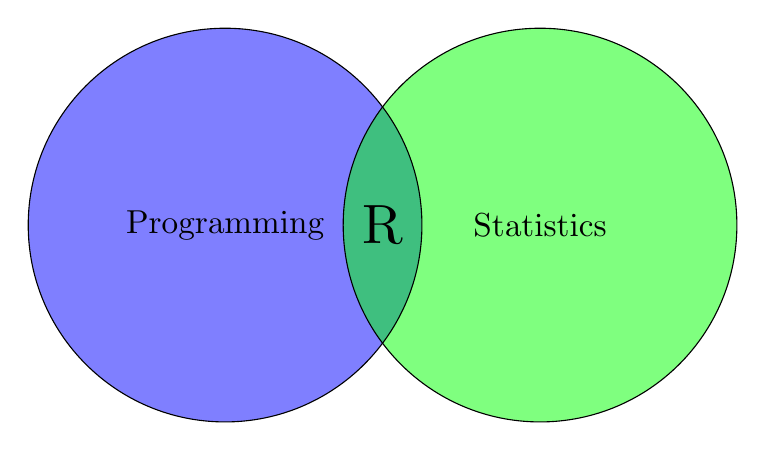
\begin{tikzpicture}
  \begin{scope}

    % The transparency:
    \begin{scope}[fill opacity=0.5]
      \fill[blue] (-2,0) circle (2.5);
      \fill[green] (2,0) circle (2.5);
    \end{scope}
    
    % letterings and missing pieces:
    \draw[align=center] (-2,0) circle (2.5) node[scale=1.2] {Programming};
    \draw[align=center] (2,0) circle (2.5) node[scale=1.2] {Statistics};
 		\draw (0,0) node[scale=2] {R};
 		
  \end{scope}
\end{tikzpicture}\\~\\
R is both... this creates a steep learning curve.
\end{center}
\end{frame}


%%%%%%
\begin{frame}[t]{What is \includegraphics[width=0.07\textwidth]{Rlogo.jpg} \hspace{0.2em}? }
\vspace{-0.1in}
\begin{columns}
\begin{column}{0.4\textwidth}
R is becoming the statistical software of choice\\~\\
Plot of Google scholar hits over time for different software packages
[\href{http://r4stats.com/articles/popularity/}{r4stats.com}]
\end{column}
\begin{column}{0.5\textwidth}
\begin{center}
\includegraphics[width=1.1\textwidth]{r_google.png}
\end{center}
\end{column}
\end{columns}
\end{frame}

%%%%%%
\begin{frame}[t]{What is \includegraphics[width=0.07\textwidth]{Rlogo.jpg} \hspace{0.2em}? }
\vspace{-0.1in}
\begin{columns}
\begin{column}{0.4\textwidth}
R is becoming the statistical software of choice\\~\\
Exponential growth in number of contributed packages
[\href{http://r4stats.com/articles/popularity/}{r4stats.com}]
\end{column}
\begin{column}{0.5\textwidth}
\begin{center}
\includegraphics[width=1.1\textwidth]{r_package.png}
\end{center}
\end{column}
\end{columns}
\end{frame}

%%%%%%
\begin{frame}{What's possible with \includegraphics[width=0.07\textwidth]{Rlogo.jpg} \hspace{0.2em}? }
R is incredibly flexible, if you want something done, someone else has written the code...\\~\\
\onslide<2->
R is open-source software, which mean it's free and is supported by a large network of contributors - the Comprehensive R Network [\href{http://cran.us.r-project.org/}{CRAN}]\\~\\
\onslide<3->
CRAN is a collection of sites which carry identical material, consisting of the R distribution(s), the contributed extensions, documentation for R, and binaries [\href{http://cran.us.r-project.org/faqs.html}{R FAQ}]\\~\\
\onslide<4->
Basically a repository of R utilities that others have written \onslide<5->- the \href{http://cran.r-project.org/web/views/}{CRAN task views} contain descriptions of contributed packages by category
\end{frame}

%%%%%%
\begin{frame}[t]{What's possible with \includegraphics[width=0.07\textwidth]{Rlogo.jpg} \hspace{0.2em}? }
\begin{center}
\includegraphics{cran_view1.png}
\end{center}
\end{frame}

%%%%%%
\begin{frame}[t]{What's possible with \includegraphics[width=0.07\textwidth]{Rlogo.jpg} \hspace{0.2em}? }
\begin{center}
\includegraphics{cran_view2.png}
\end{center}
\end{frame}

%%%%%%
\begin{frame}[t,fragile]{What's possible with \includegraphics[width=0.07\textwidth]{Rlogo.jpg} \hspace{0.2em}? }
R has a base package that is included in installation, others are downloaded as needed\\~\\
<<echo=true,eval=false>>=
install.packages('newpackage')
@
\vspace{0.2in}
The base package will be sufficient for most of your needs - includes arithmetic, input/output, basic programming support, graphics, etc.\\~\\
Contributed packages will meet your other needs - now exceed 4000
\end{frame}

%%%%%%
\begin{frame}[t,fragile]{What's possible with \includegraphics[width=0.07\textwidth]{Rlogo.jpg} \hspace{0.2em}? }
<<eval=false,echo=true>>=
demo(package = .packages(all.available = TRUE))
@
List of demonstrations with available packages - examples from ggplot2 package
\begin{columns}
\begin{column}{0.5\textwidth}
\begin{center}
\includegraphics[width=\textwidth]{ggplot1.png}
\end{center}
\end{column}
\begin{column}{0.5\textwidth}
\begin{center}
\includegraphics[width=\textwidth]{ggplot3.png}
\end{center}
\end{column}
\end{columns}
\end{frame}

%%%%%%
\begin{frame}[t,fragile]{What's possible with \includegraphics[width=0.07\textwidth]{Rlogo.jpg} \hspace{0.2em}? }
<<eval=false,echo=true>>=
demo(package = .packages(all.available = TRUE))
@
List of demonstrations with available packages - examples from ggplot2 package
\begin{columns}
\begin{column}{0.5\textwidth}
\begin{center}
\includegraphics[width=\textwidth]{ggplot2.png}
\end{center}
\end{column}
\begin{column}{0.5\textwidth}
\begin{center}
\includegraphics[width=\textwidth]{ggplot4.png}
\end{center}
\end{column}
\end{columns}
\end{frame}

\section{Basics}
%%%%%%
\begin{frame}[t]{\includegraphics[width=0.07\textwidth]{Rlogo.jpg} \hspace{0.01in} basics}
Installation - visit \href{http://cran.us.r-project.org/}{r-project.org} and follow directions
\centerline{\includegraphics{download.png}}
\end{frame}

%%%%%%
\begin{frame}[t]{\includegraphics[width=0.07\textwidth]{Rlogo.jpg} \hspace{0.01in} basics}
Or visit \href{http://pbil.univ-lyon1.fr/Rweb/}{Rweb} for an online version (not recommended)
\centerline{\includegraphics{rweb.png}}
\end{frame}

%%%%%%
\begin{frame}[t]{\includegraphics[width=0.07\textwidth]{Rlogo.jpg} \hspace{0.01in} basics}
A text editor is highly recommended, e.g. \href{http://www.rstudio.com/}{RStudio}\\~\\
\centerline{\includegraphics[width=0.65\textwidth]{Rstudio.png}}
\end{frame}

%%%%%%
\begin{frame}[t]{\includegraphics[width=0.07\textwidth]{Rlogo.jpg} \hspace{0.01in} basics}
How is R different from Excel? \onslide<2-> R is a command-line interface\\~\\
\centerline{\includegraphics[width=0.7\textwidth]{command_line.png}}
\onslide<3>
\centerline{\emph{What next??}}
\end{frame}

%%%%%%
\begin{frame}[fragile]{\includegraphics[width=0.07\textwidth]{Rlogo.jpg} \hspace{0.01in} basics}
Lines of code are executed by R at the prompt (\textit{\texttt{>}})\\~\\
\onslide<2>
Enter the code and press enter, the output is returned\\~\\
<<echo=T,results=tex>>=
print('hello world!')
2+2
(2+2)/4
rep("a",4)
@

\end{frame}

%%%%%%
\begin{frame}[fragile]{\includegraphics[width=0.07\textwidth]{Rlogo.jpg} \hspace{0.01in} basics}
A disadvantage of code is that everything entered must be 100 \% correct
\begin{Schunk}
\begin{Sinput}
> 2+2a
\end{Sinput}
\begin{Soutput}
Error: unexpected symbol in "2+2a"
\end{Soutput}
\begin{Sinput}
> a
\end{Sinput}
\begin{Soutput}
Error: object 'a' not found
\end{Soutput}
\end{Schunk}
\onslide<2>
\vspace{0.2in}
But this enables a complete documentation of your workflow... \\~\\
...your code is a living document of your analyses.
\end{frame}

%%%%%%
\begin{frame}[t,fragile]{\includegraphics[width=0.07\textwidth]{Rlogo.jpg} \hspace{0.01in} basics}
Assigning data to R objects is critical for analysis\\~\\
\onslide<2>
Assignment is possible using \textit{\texttt{<-}} or \textit{\texttt{=}}\\~\\
<<eval=true,echo=true>>=
a<-1
2+a
a=1
2+a
a=2+2
a/4
@
\end{frame}

%%%%%%
\begin{frame}[t,fragile]{\includegraphics[width=0.07\textwidth]{Rlogo.jpg} \hspace{0.01in} basics}
Assigning data to R objects is critical for analysis\\~\\
More complex assignments are possible\\~\\
<<eval=true,echo=true>>=
a<-c(1,2,3,4)
a
a<-seq(1,4)
a
a<-c("a","b","c")
a
@
\end{frame}

%%%%%%
\begin{frame}[fragile]{\includegraphics[width=0.07\textwidth]{Rlogo.jpg} \hspace{0.01in} basics}
Anatomy of a function - functions perform tasks for you, much like in Excel
\begin{center}
\Large
function(arguments)
\end{center}
\onslide<2>
<<eval=true,echo=true>>=
c(1,2) #concatenate function
mean(c(1,2)) #mean function
seq(1,4) #create a sequence of values
@
\end{frame}

%%%%%%
\begin{frame}[fragile,t]{\includegraphics[width=0.07\textwidth]{Rlogo.jpg} \hspace{0.01in} basics}
Understanding classes of R \href{http://cran.r-project.org/doc/manuals/r-release/R-lang.html#Vector-objects}{objects} is necessary for analysis \\~\\
An object is any variable of interest that you want to work with\\~\\
The class defines the type of information the object contains\\~\\
\onslide<2>
Most common are `numeric' or `character' classes \\~\\
<<echo=true,eval=true>>=
class(1)
class("1")
@
\vspace{0.2in}
\pause
`Factors' are also common, define categorical variables
\end{frame}

%%%%%%
\begin{frame}[fragile,t]{\includegraphics[width=0.07\textwidth]{Rlogo.jpg} \hspace{0.01in} basics}
Understanding classes of R \href{http://cran.r-project.org/doc/manuals/r-release/R-lang.html#Vector-objects}{objects} is necessary for analysis \\~\\
The classes of an object defines a protocol for evaluating or organizing variables\\~\\
For example, we cannot add add two objects with different classes:\\~\\
<<echo=true,eval=false>>=
'1' + 1
@
\begin{Schunk}
\begin{Soutput}
Error in "1" + 1 : non-numeric argument to binary operator
\end{Soutput}
\end{Schunk}
\end{frame}

%%%%%%
\begin{frame}[fragile]{\includegraphics[width=0.07\textwidth]{Rlogo.jpg} \hspace{0.01in} basics}
Objects (and their classes) can be stored in the computer's memory in different ways - aka the workspace for your R session\\~\\
Most common structures are `vectors' and `data.frames'\\~\\
\onslide<2->
Vectors are a collection of objects of the same class (e.g., a column in a table), whereas a data frame is analogous to a table with rows and columns (e.g., collection of vectors)
\onslide<3->
\begin{columns}[t]
\begin{column}{0.45\textwidth}
<<echo=true,eval=true>>=
a<-c(1,2)
a
b<-c("a","b")
b
@
\end{column}
\onslide<4->
\begin{column}{0.45\textwidth}
<<>>=
c<-data.frame(a,b)
c
@
\end{column}
\end{columns}
\end{frame}

%%%%%%
\begin{frame}[t,fragile]{\includegraphics[width=0.07\textwidth]{Rlogo.jpg} \hspace{0.01in} basics}
How are data imported into R?\\~\\
R needs to know where the data are located on your computer:\\~\\
<<echo=true,results=tex,eval=false>>=
setwd("C:/projects/my_data/")
@
\vspace{0.2in}
This establishes a `working directory' for data import/export\\~\\
\onslide<2>
R can import almost any type of data but `spreadsheet' or text-based files are most common \\~\\
\end{frame}

%%%%%%
\begin{frame}[t,fragile]{\includegraphics[width=0.07\textwidth]{Rlogo.jpg} \hspace{0.01in} basics}
How are data imported into R?\\~\\
R can import Excel data using the RODBC package, but this is not simple\\~\\
\onslide<2>
The easiest approach is to format data in Excel then export to a .csv or .txt file
\begin{columns}
\begin{column}{0.43\textwidth}
\begin{center}
\includegraphics{my_dat.png}
\end{center}
\end{column}
\begin{column}{0.66\textwidth}
\begin{center}
\includegraphics{save_as.png}
\end{center}
\end{column}
\end{columns}
\end{frame}

%%%%%%
\begin{frame}[t,fragile]{\includegraphics[width=0.07\textwidth]{Rlogo.jpg} \hspace{0.01in} basics}
How are data imported into R?\\~\\
Use the read.table or read.csv functions to import the data, must be in your working directory\\~\\
\onslide<2>
<<echo=true,eval=true>>=
dat<-read.csv("my_data.csv",header=T)
dat
@
\end{frame}

%%%%%%
\begin{frame}[t,fragile]{\includegraphics[width=0.07\textwidth]{Rlogo.jpg} \hspace{0.01in} basics}
How are data imported into R?\\~\\
Use the read.table or read.csv functions to import the data, must be in your working directory\\~\\
<<echo=true,eval=true>>=
dat<-read.table("my_data.csv",sep=',',header=T)
dat
@
\end{frame}

%%%%%%
\begin{frame}[t,fragile]{\includegraphics[width=0.07\textwidth]{Rlogo.jpg} \hspace{0.01in} basics}
Imported data can be viewed several ways, view the whole object or parts \\~\\
Rows or columns can be obtained by indexing with brackets separated by a comma: data[row,column]
\begin{columns}[t]
\onslide<2->
\begin{column}{0.45\textwidth}
<<echo=true>>=
dat
@
\end{column}
\onslide<3>
\begin{column}{0.45\textwidth}
<<>>=
dat[1,] #row 1
dat[,2] #column 2
dat[4,1] #row 4, column 1
@
\end{column}
\end{columns}
\end{frame}

%%%%%%
\begin{frame}[t,fragile]{\includegraphics[width=0.07\textwidth]{Rlogo.jpg} \hspace{0.01in} basics}
Imported data can be viewed several ways, view the whole object or parts \\~\\
Access using column names or the attach function
\begin{columns}[t]
\begin{column}{0.49\textwidth}
<<echo=true>>=
dat$Value
dat[,'Value']
@
\end{column}
\begin{column}{0.49\textwidth}
<<>>=
attach(dat)
Value
@
\end{column}
\end{columns}
\vspace{0.3in}
\onslide<2>
Vectors can be indexed similarly as data frames\\~\\
<<>>=
Value[2]
@
\end{frame}

%%%%%%
\begin{frame}[t,fragile]{\includegraphics[width=0.07\textwidth]{Rlogo.jpg} \hspace{0.01in} basics}
Where to go for help?\\~\\
\begin{itemize}
\addtolength{\itemsep}{0.08in}
\item A user-friendly \href{http://www.statmethods.net/}{intro to R} \pause
\item Several good introductory texts are available - Zuur et al. 2009. A Beginner's Guide to R. Springer. \pause
\item \href{http://cran.r-project.org/doc/contrib/Short-refcard.pdf}{R cheatsheet} \pause
\item Google is your friend \pause
\item Help files for each function using `?function' - may or may not be helpful \pause
\item An \href{http://cran.r-project.org/doc/manuals/R-intro.html}{intro to R} - very detailed
\item Ask us!
\end{itemize}
\end{frame}

% \begin{frame}[shrink]{References}%[t,allowframebreaks]{References}
% \scriptsize
% \setbeamertemplate{bibliography item}{}
% \bibliographystyle{C:/Projects/LaTeX/bibtex_bst/apalike_mine}
% \bibliography{C:/Projects/LaTeX/ref_diss}
% \end{frame}

\end{document}